\chapter{Interpreting a Logistic Regression Model \label{chapter:logreg}}

This chapter is similar to Chapter~\ref{chapter:linreg} but focuses on logistic regression models. As we saw in Chapter~\ref{chapter:linreg}, linear regression models are used in situations where the outcome of a supervised learning problem, $y$, follows a normal distribution, conditional on the values of the predictors. \textbf{Logistic regression} models, in contrast, handle situations where the outcome, $y$, is binary: either 0 or 1. We first encountered these models as examples of classification algorithms in Chapter~\ref{chapter:classification}. Because of their popularity in the clinical domain, it's important to understand how these models are fit and how to interpret the summary output produced by software. 

Unfortunately, a full understanding of logistic regression requires knowledge of maximum likelihood estimation. We will, therefore, skip over some of the details until we've had more time to explore this topic. 

%%%%%%%%%%%%%%%%%%%%%%%%%%%%%%%%%%%%%%%%%%%%%%%%%%%%%%%%%%%%%%%%%%%%%%%%%%%%%%%%

\section{ER Readmissions Example from Chapter~\ref{chapter:classification} \label{sect:eragain}}

In Chapter~\ref{chapter:classification}, we saw an example where information about two predictors -- a disease severity score ($x_1$) and a social determinants score ($x_2$) -- was used to predict a binary outcome: whether a patient would be readmitted to the ER within 30 days of discharge. We tried three different supervised learning algorithms, one of which was a logistic regression model (Section~\ref{ssect:logreg}). The output from that model is repeated below.

\begin{center}
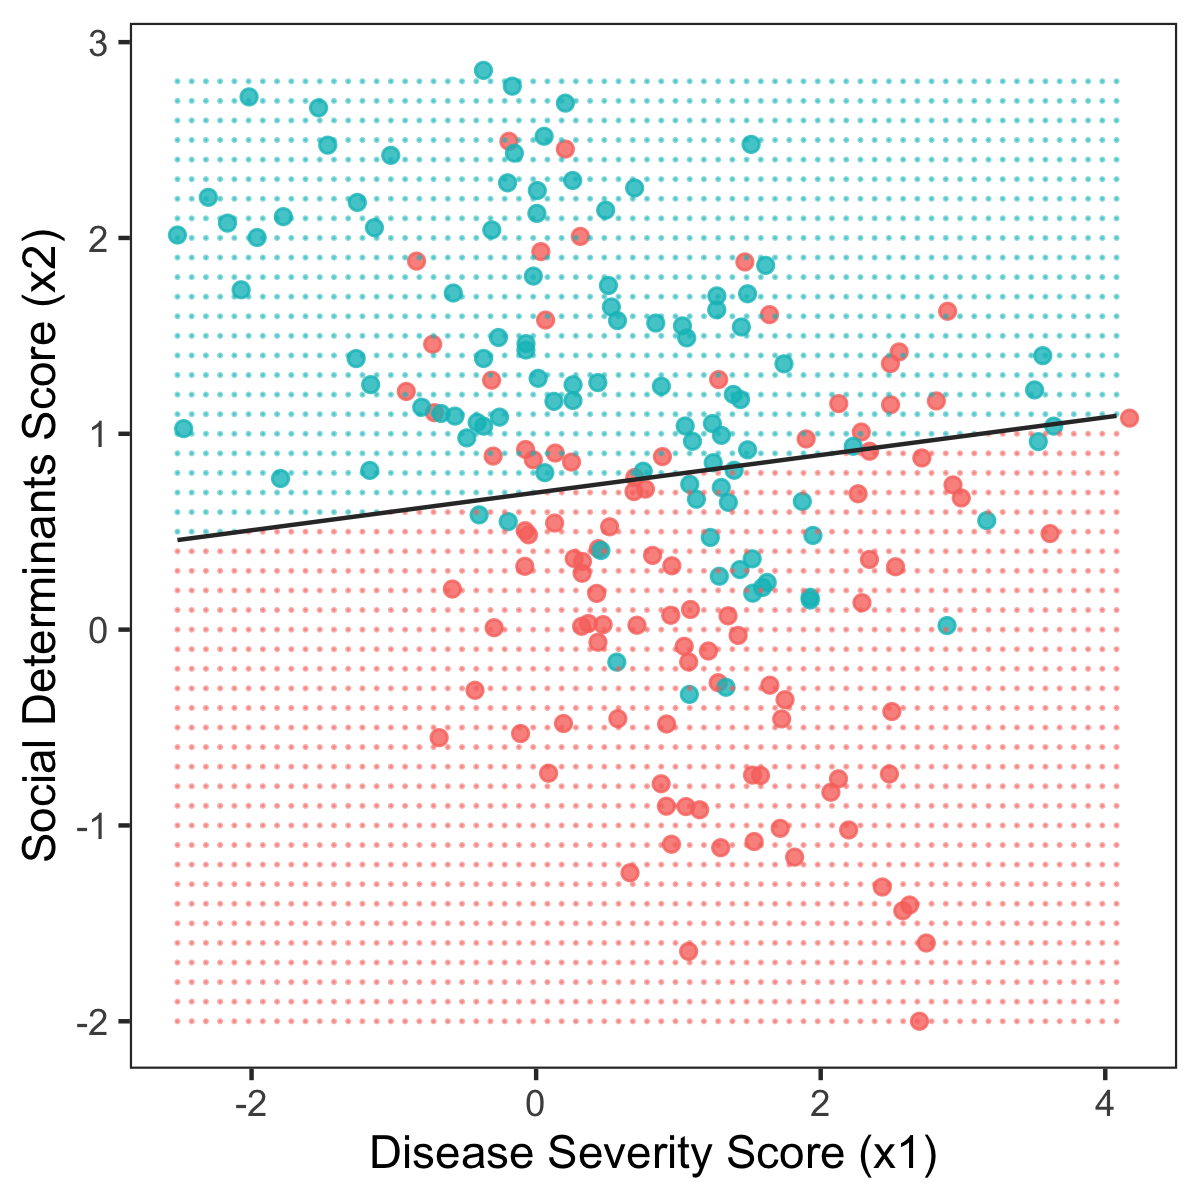
\includegraphics[width=0.35\textwidth]{img/esl-logistic.png}
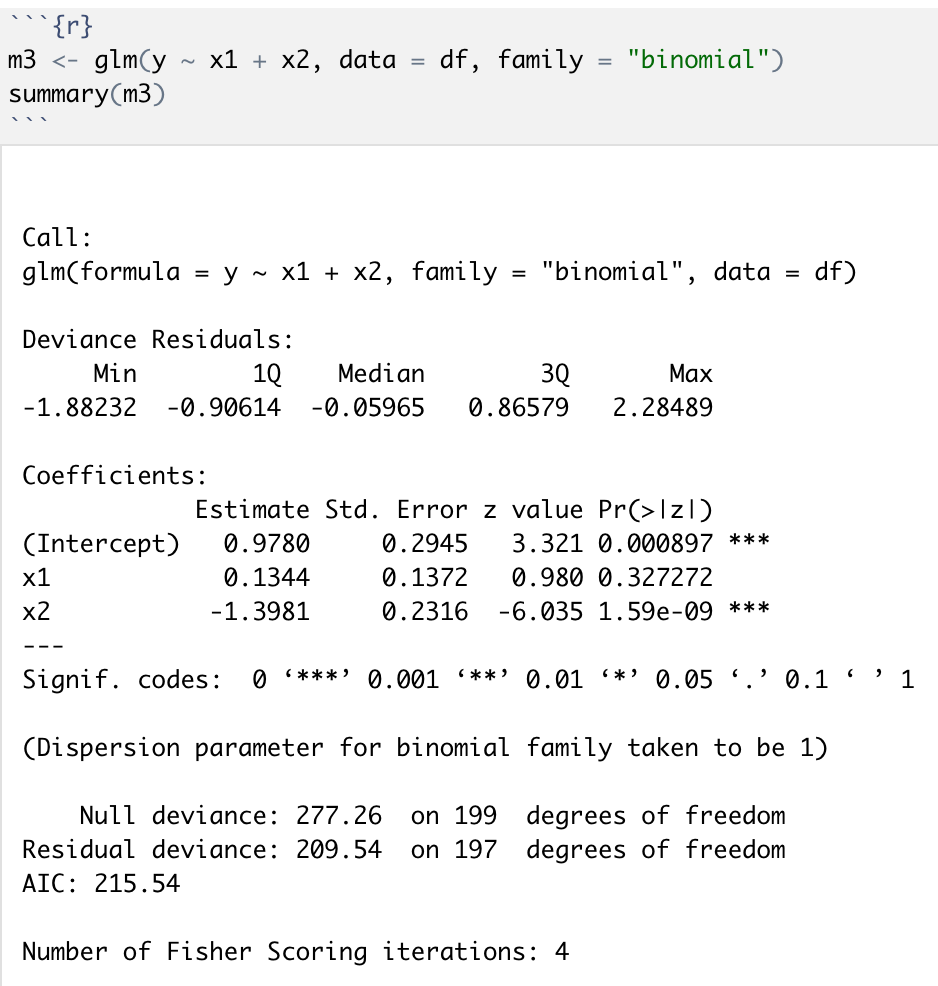
\includegraphics[width=0.64\textwidth]{img/glm-binomial-example.png}
\end{center}

%%%%%%%%%%%%%%%%%%%%%%%%%%%%%%%%%%%%%%%%%%%%%%%%%%%%%%%%%%%%%%%%%%%%%%%%%%%%%%%%

\section{Understanding the Model Summary}

A logistic regression model looks like this (see also Section~\ref{ssect:logreg}):
\begin{equation} \log \frac{\mu}{1-\mu} = \beta_0 + \beta_1 x_1 + \dots + \beta_p x_p \label{eqn:logistic} \end{equation}
where $\mu$ is the mean of the Bernoulli distribution (see Section~\ref{sect:bernoulli}) governing our binary outcome, $y$; in other words, it is the probability that $y = 1$. 

You will note that there is no independent error term here as there was in linear regression. That's because the variance and mean of a Bernoulli distribution are coupled and depend only on $\mu$ (again, see Section~\ref{sect:bernoulli}). 
\vspace{3mm}

\begin{question}{question:logreglink}
In logistic regression, $\mu$ itself is not equal the sum of the predictors; instead, the \textbf{logit} of $\mu$ is their sum. Based on what you know about $\mu$, why is a logistic regression model not of the form
$$ \mu = \beta_0 + \beta_1 x_1 + \dots + \beta_p x_p \text{?}$$
We will explore this further in Chapter~\ref{chapter:glms}.
\end{question}

\begin{question}{}
The decision boundary in logistic regression (see picture above) occurs where the sum of the linear predictors, $\beta_0 + \beta_1 x_1 + \dots + \beta_p x_p$, is zero. What value of $\mu$ does this correspond to? Why does this make sense, intuitively?
\end{question}

\subsection{The Call}

The first line of the output repeats the call you made to the \verb|glm| function in R to fit the model. The \texttt{glm} package fits a variety of different generalized linear models using maximum likelihood estimation (see Chapter~\ref{chapter:mlebasics}; this will also be discussed in more detail in Chapter~\ref{chapter:glms}). The \texttt{family = "binomial"} argument tells the function to fit a logistic regression model.

\subsection{Coefficients and Standard Errors}

Logistic regression models, like other GLMs, are fit using maximum likelihood (see Chapter~\ref{chapter:mlebasics} for a brief introduction). We will skip most of the details for now, but you can gain intuition by staring at Equation~\ref{eqn:logistic}. This equation says that the model's predicted value of $\mu$, the probability that the outcome will be positive ($y=1$), is controlled by the values of the predictors and their coefficients $\beta_0, \dots, \beta_p$. 

By adjusting the values of the $\beta$s, the model causes $\mu$ to be high in regions of the feature space where $y=1$ and low where $y=0$. The values of the $\beta$s that do this the best are called the \textbf{maximum likelihood estimates}, and they are the coefficients shown in the model output.

As with linear regression, a full understanding of the standard errors requires matrix multiplication. However, they are related to the same factors that drive the standard errors in linear regression: (1) the spread of the values of the corresponding covariate about its mean (more spread will decrease the standard error) and (2) correlations between that covariate and other covariates in the model (tighter correlations will increase the standard error).
\vspace{5mm}

\begin{question}{}
Looking at the form of the logistic regression model
$$ \log \frac{\mu}{1-\mu} = \beta_0 + \beta_1 x_1 + \dots + \beta_p x_p $$
what does the value of each of the $\beta$s mean? What is $\beta_j$ telling us about how $y$ varies with the predictor $j$, all else being equal?
\end{question}

\begin{question}{}
The \textbf{odds} of something happening are defined as $\mu/(1-\mu)$, where $\mu$ is the probability that the thing occurs. In our example model, we are interested in the odds that $y=1$ (the patient is readmitted). Does a unit increase in $x_1$ (disease severity score) increase or decrease the odds that a patient will be readmitted? What about $x_2$ (social determinants score)? 
\end{question}

\begin{question}{}
What are the odds of readmission for a patient with:
\begin{enumerate}[label=(\alph*)] 
\item $x_1 = 0.1$ and $x_2 = 0.3$?
\item $x_1 = 0.1$ and $x_2 = -1.3$?
\item $x_1 = 1.1$ and $x_2 = 0.3$?
\end{enumerate}
\end{question}

\subsection{Hypothesis Tests of Coefficients}

Just as in linear regression, we can use our coefficients and standard errors to perform a hypothesis test on each regression coefficient, $\beta_j$, against the null hypothesis that $\beta_j = 0$ (the predictor $x_j$ has no effect on the outcome). In logistic regression, the quantity $\hat{\beta_j}/\text{se}(\hat{\beta}_j)$ will follow a normal distribution under the null.
\vspace{3mm}

\begin{question}{question:nulllogregexample}
Below are the null distributions for the hypothesis tests of our three regression coefficients, $\beta_0$, $\beta_1$, and $\beta_2$. In each graph, the maximum likelihood estimate of the coefficient is shown as a vertical dashed line. Based on these graphs, can you tell why the $p$-values for $\beta_0$ and $\beta_2$ are low and the one for $\beta_1$ is high? What is the intuition behind this?
\begin{center}
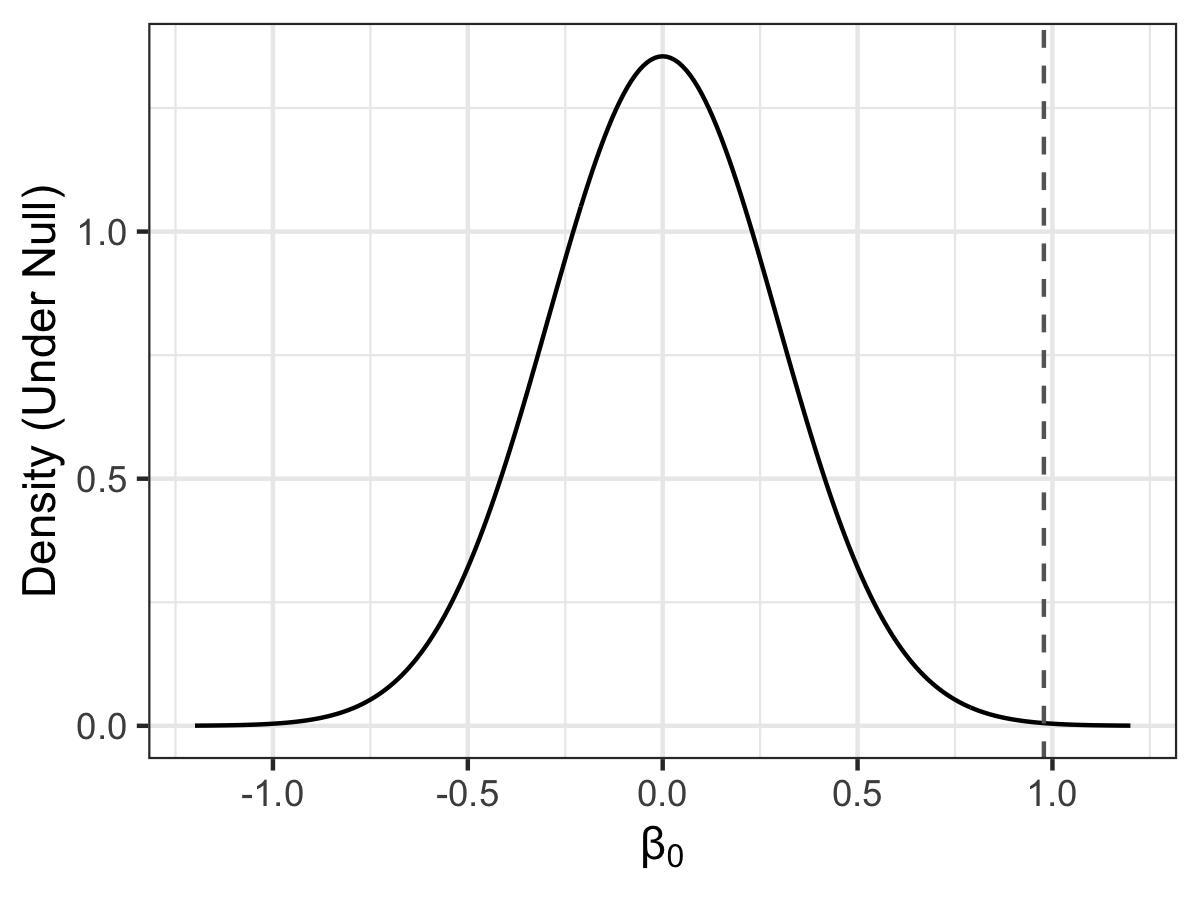
\includegraphics[width=0.45\textwidth]{img/logreg-example-beta-0.png}
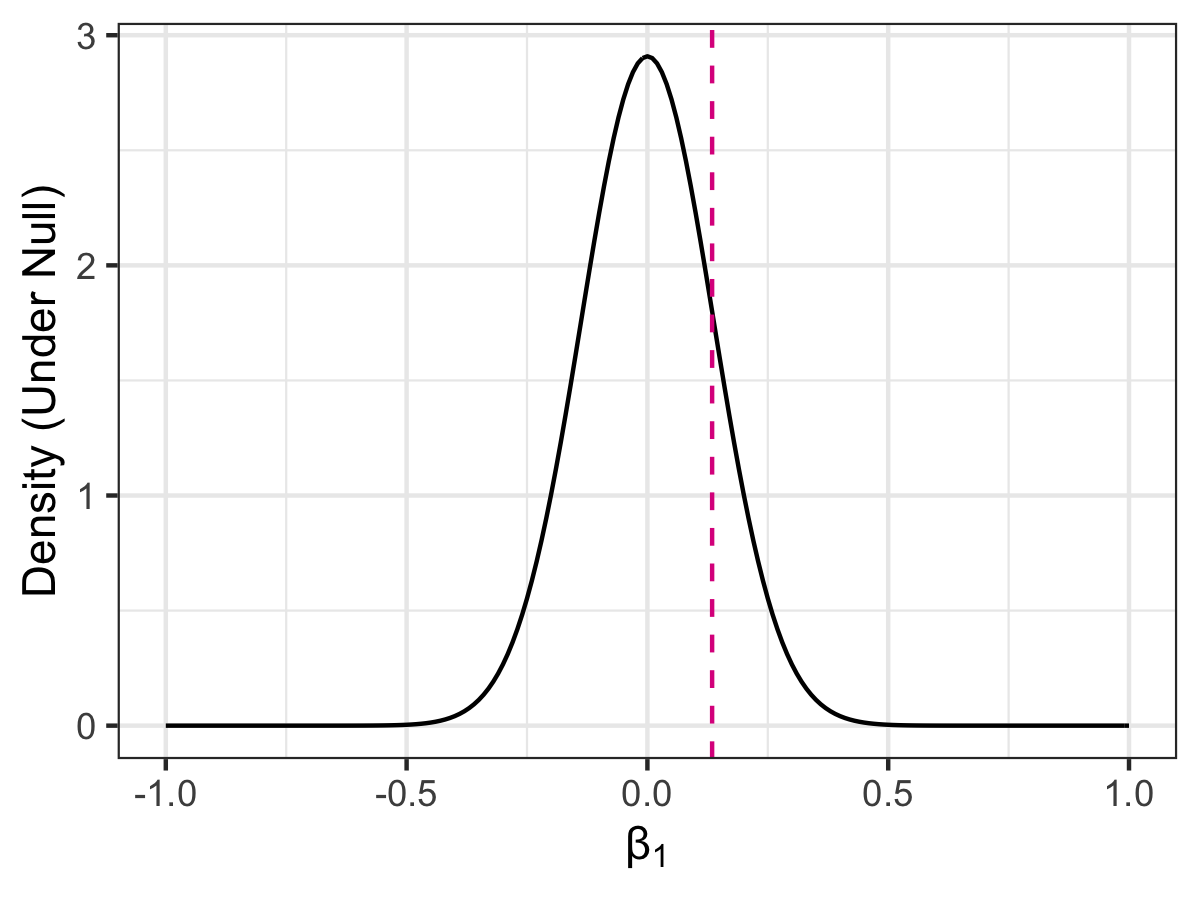
\includegraphics[width=0.45\textwidth]{img/logreg-example-beta-1.png}
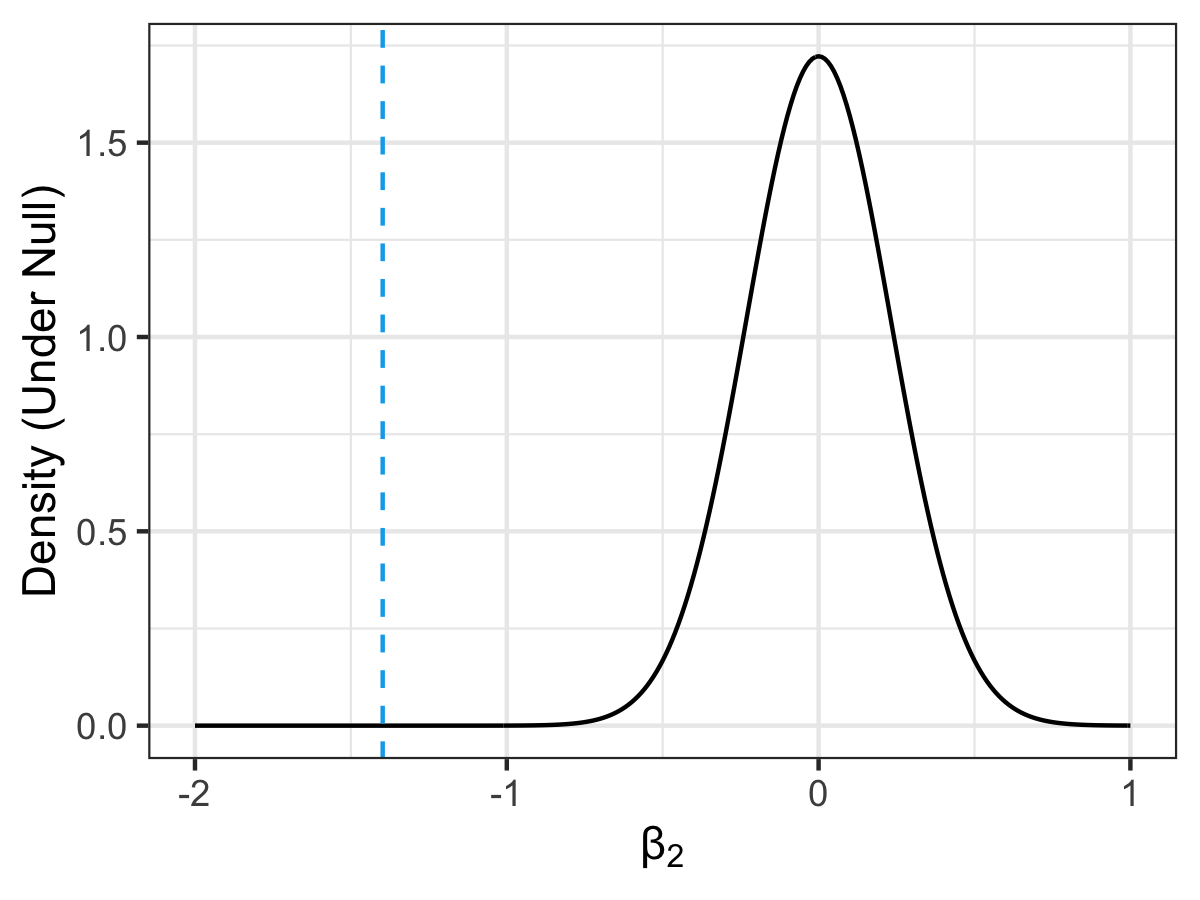
\includegraphics[width=0.45\textwidth]{img/logreg-example-beta-2.png}
\end{center}
\end{question}

\subsection{Deviance and Deviance Residuals}

The \textbf{deviance} (called \textbf{residual deviance} in the model output) plays a role in GLMs akin to that of the residual standard error in linear regression; it is a measure of the residual variation in the outcome not explained by the model. The \textbf{null deviance} is the deviance for a model that only includes an intercept. Under the null hypothesis that all of the $\beta$s are zero except the intercept (i.e, a model with no predictors explains the data as well as our model), the difference
$$ \text{null deviance} - \text{residual deviance} $$
is distributed as $\chi^2_p$, a chi-squared distribution (see Section~\ref{sect:chisqdist}) with $p$ degrees of freedom, where $p$ is the number of predictors.
\vspace{5mm}

\begin{question}{}
This test is a hypothesis test of the null hypothesis that a model with no predictors fits our data as well as our model, where goodness of fit is measured by the deviance (lower is better). What is this hypothesis test akin to in the linear regression model output?
\end{question}

\begin{question}{}
The difference in null and residual deviances in this case is $67.72$. It follows a $\chi^2_2$ distribution under the null. A plot of the $\chi^2_2$ distribution and our test statistic is shown below. What do these findings indicate about the $p$-value of this goodness of fit test and what does it mean?
\begin{center}
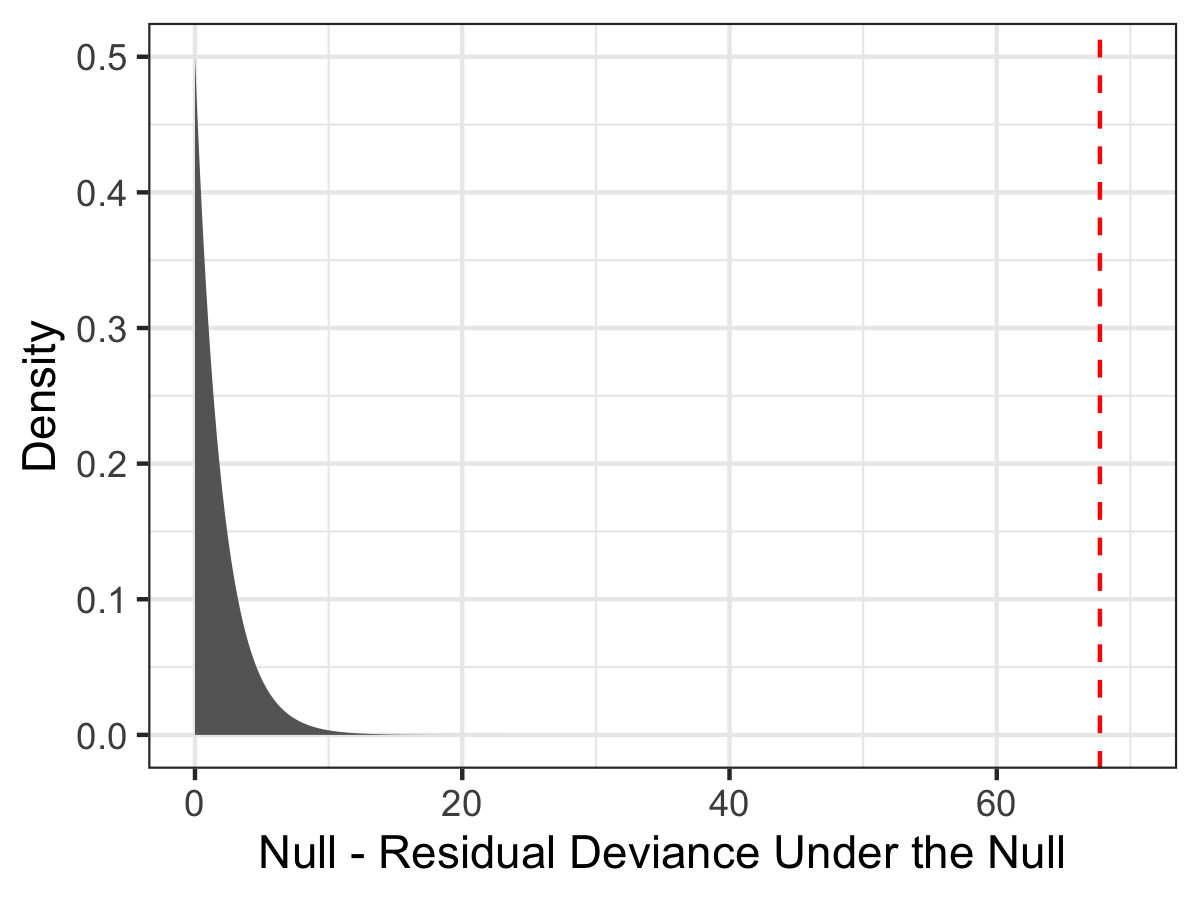
\includegraphics[width=0.7\textwidth]{img/logreg-example-goodness-of-fit-test.png}
\end{center}
\end{question}

In the GLM context, there are multiple types of residual (more on this later). \textbf{Deviance residuals} quantify the contributions of the individual samples to the deviance. Unfortunately, the output from \texttt{glm} is confusing because what \texttt{glm} calls a deviance residual in the model summary is actually something called a \textbf{working residual}. We will ignore this part of the output until we understand more about the inner workings of GLMs. 

%%%%%%%%%%%%%%%%%%%%%%%%%%%%%%%%%%%%%%%%%%%%%%%%%%%%%%%%%%%%%%%%%%%%%%%%%%%%%%%%

\section{Example: Low Birthweight Dataset \label{sect:lowbwt}}

The goal of this study was to identify risk factors associated with giving birth to a low birth weight baby (a baby weighing less than 2500 grams). Infant mortality rates and birth defect rates are very high for low birth weight babies. A woman's behavior during pregnancy (including diet, smoking habits, and receiving prenatal care) can greatly alter the chances of carrying the baby to term and, consequently, of delivering a baby of normal birth weight.

Data were collected on 189 women, 59 of which had low birth weight babies and 130 of which had normal birth weight babies\footnote{SOURCE: Hosmer and Lemeshow (2000) \emph{Applied Logistic Regression: Second Edition}. Data were collected at Baystate Medical Center, Springfield, Massachusetts during 1986.}.

\begin{center}
\texttt{ \small
\begin{tabular}{ll}
\toprule
LOW & Low birth weight (0 = birth weight $\geq$ 2500 g;\\
& 1 = birth weight $< 2500$ g) \\
AGE & Age of mother in years \\
LWT & Mother's weight in pounds at last menstrual period \\
RACE & Race (1 = white, 2 = black, 3 = other) \\
SMOKE & Smoking status during pregnancy (1 = yes, 0 = no) \\
PTL & History of premature labor (0 = none, 1 = one, etc.) \\
HT & History of hypertension (0 = no, 1 = yes) \\
UI & Presence of uterine irritability (0 = no, 1 = yes) \\
FTV & Number of physician visits during the first trimester \\
BWT & Birth weight in grams \\
\bottomrule
\end{tabular}
}
\end{center}

We will build a model that predicts the value of \texttt{LOW} based on all of the other covariates except, of course, \texttt{BWT}. (Why not use \texttt{BWT}?) 

\begin{center}
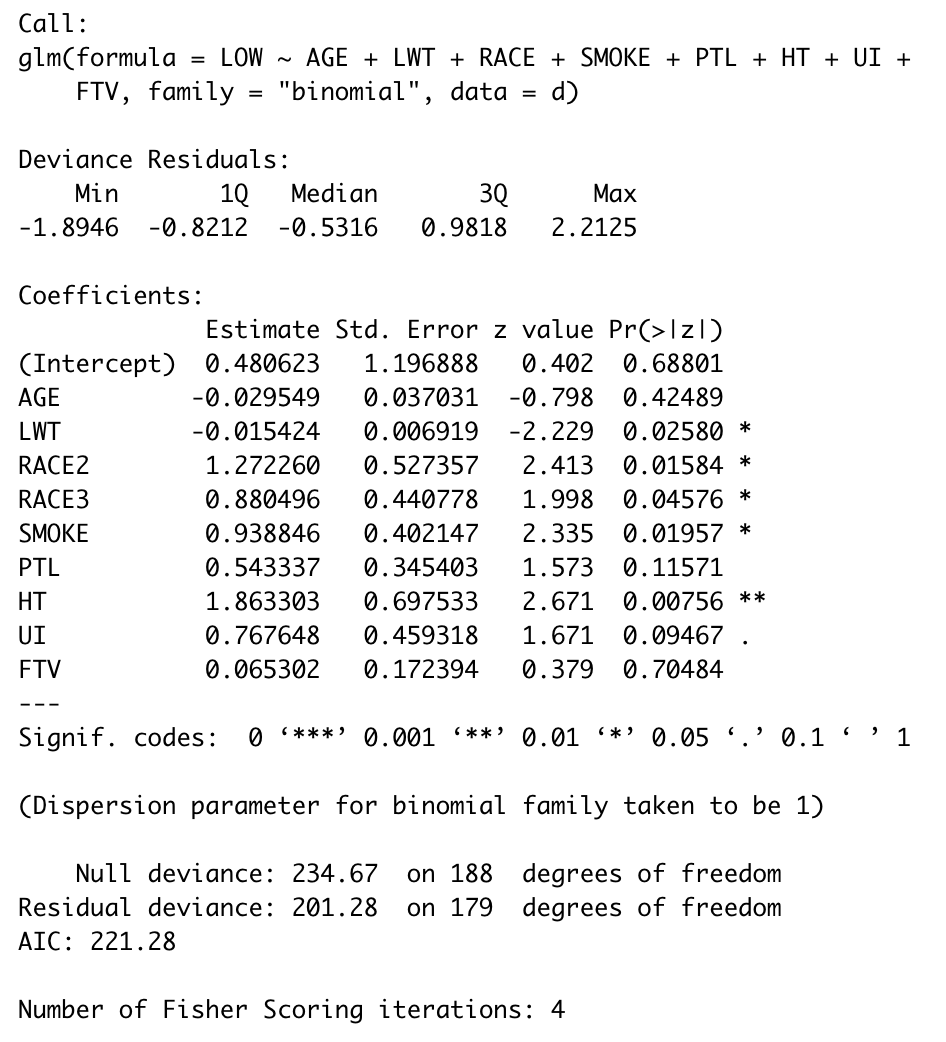
\includegraphics[width=0.7\textwidth]{img/logreg-low-bwt-example-model.png}
\end{center}

\begin{question}{}
In this model, is the effect of one predictor (say, \verb|AGE|) impacted by the value(s) of any of the other predictor(s)? How does this differ from the other classification algorithms we've seen (KNN and decision trees)? What are the advantages and disadvantages of this choice? 
\end{question}

\begin{question}{}
Comment on how the variable \texttt{RACE} enters into the model here. Does this make sense in light of what that variable means and how it potentially interacts with the other study variables?
\end{question}

\begin{question}{}
Interpret the values of each of these coefficients. Based on the coefficient values and their standard errors, which predictor(s) do you think have the greatest impact on whether or not a woman has a low birthweight baby? 
\end{question}
